%!TEX root=../../template.tex
Macroscopically, the approach to the \gls{RQ} was conducted by working
with two hypothesis:
\begin{description}
    \item[First Hypothesis:] The definition of a particular set of
        algorithmically defined projections in such a manner that they
        might be used for tomographic reconstruction of column densities
        of trace gases in the atmosphere, in a given \gls{ROI};
    \item[Second Hypothesis:] We can retrieve the column density for a
        given trace gas (or set of trace gases) between two points by
        performing a spectral measurement in both of these points in the
        same direction and subtracting them one from the other.
\end{description}

Testing the first hypothesis implies the design of a whole system and
requires a very diverse and multidisciplinary approach. I have already
covered that the system should be drone-mounted. But which drone? And
what is the collection system? And then again, what trajectory shall
this drone adopt? Do we know it works?

Figure~\ref{fig:general_system_schematic} is a general diagram of the
envisaged solution. Section~\ref{sec:methods_first_hypothesis} aims to
provide a complete description of how I have arrived at the system that
I propose, and of the subsystems that comprise it.
Subsection~\ref{sub:methods_uav} is dedicated to the description of the
drone and its subsystems, the \textcolor{blue}{blue} box in the figure,
Subsection~\ref{sub:methods_collection} is about the particularities of
the collection system and corresponds to the \textcolor{red}{red} box in
the figure. The ground station is addressed in
Subsection~\ref{sub:methods_ground_station}, which is the
\textcolor{orange}{orange} box in the figure. Finally, the trajectory
simulation platform (\textcolor{green}{green} box) is the matter of
Subsection~\ref{sub:methods_tomosim}.

\begin{figure}[htpb]
    \centering
    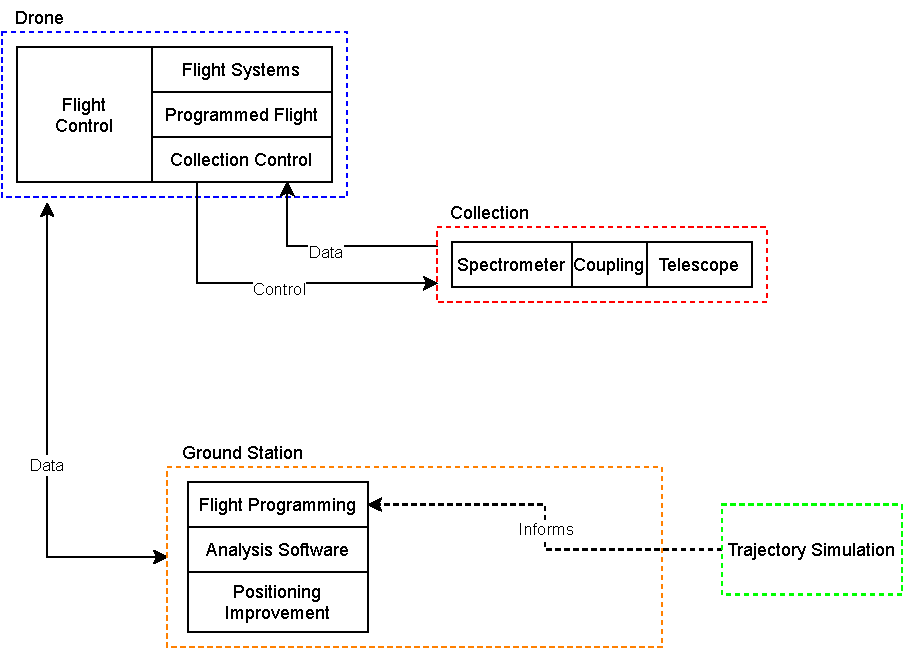
\includegraphics[width=.8\textwidth]{img/pdf/general_system_diagram.pdf}
    \caption{General diagram of the atmospheric monitoring system, in an
    overview style.}%
    \label{fig:general_system_schematic}
\end{figure}

\FloatBarrier

On Section~\ref{sec:methods_second_hypothesis}, this
chapter moves to a different subject. It is aimed at the testing of the
second hypothesis. Figure~\ref{fig:measuring_over_city} is a pictorial
representation of what the proposed pollution monitoring system is
designed to (ideally) do. Our second hypothesis is based on Lambertian
theory, and tells us that one way of getting the density values in the
\gls{ROI} is to subtract whatever density is obtained to the left of the
\gls{ROI} from the density obtained by measuring on the right of the
\gls{ROI}. It is clear that, from a mathematical point of view, this is
the case. But can I measure it with current-day off-the-shelf equipment?
Subsection~\ref{sub:methods_lambertian_hypothesis} addresses the
theoretical perspective and reasoning for this idea.
Subsection~\ref{sub:methods_experiment} presents the experiment that I
have designed to test it.

\begin{figure}[htpb]
    \centering
    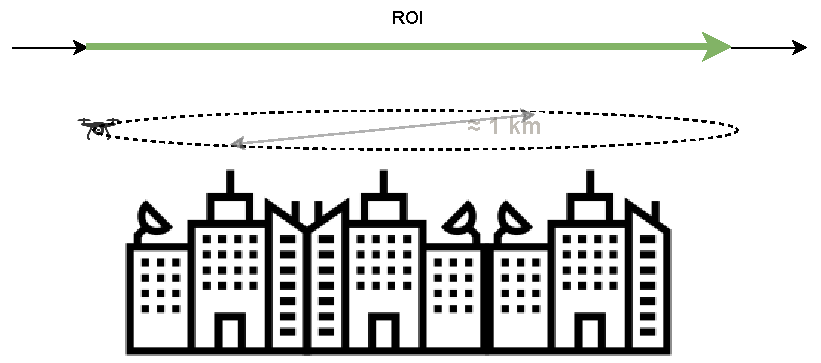
\includegraphics[width=0.8\linewidth]{img/pdf/spectralMeasurementsFromTheSide.pdf}
    \caption{Schematic representation of the intended pollution
    measurement geometry. The second hypothesis of the \gls{RQ} tells us
    that to get the \gls{ROI} we can subtract the concentrations obtained on
    the left of the \gls{ROI} from the ones obtained to the right of the
    \gls{ROI}.}%
    \label{fig:measuring_over_city}
\end{figure}

